\chapter{Objetivos}
\label{chap:objetivos}

\noindent

%TODO: Falta link tecnológico
\drop{E}{n} este capítulo se expondrán tanto el objetivo principal como los diferentes objetivos específicos del Trabajo Fin de Grado, así como las posibles limitaciones o condicionantes que se pudieran derivar de los mismos.

\section{Objetivo general}
El principal objetivo de este trabajo es implementar una herramienta de mensajería instantánea para la comunicación entre el profesorado y los padres de los alumnos específica para el contexto educativo.

Se apoyará en un \textit{backend} suministrado por la empresa Google, llamado \textit{Firebase}. Para su desarrollo se utilizará el \acf{IDE}, o Entorno de Desarrollo Integrado, en español, \textit{Android Studio}. La motivación por la que surge esta idea reside en la necesidad de disponer de una aplicación adaptada y acotada a las necesidades primordiales en la gestión de la comunicación con los padres por parte del centro educativo. Actualmente, la mayor parte de las alternativas que existen son más generalistas, orientándose a cualquier tipo de público. Por tanto, éstas incluyen funciones cuya utilidad, en el sector profesional de la docencia sería, en determinados casos, cuestionable. Adicionalmente, en la actualidad, existen diversos problemas sociales con los grupos de mensajería entre los padres y con los profesores. Estas situaciones favorecen también las intenciones de realizar una aplicación que trate de eliminarlos o, al menos, evitarlos.

\section{Objetivos específicos}
En esta sección se detallarán los objetivos específicos a completar para cumplir el objetivo general.

\subsection{Objetivo I: Gestión de los Usuarios}
Este objetivo será de especial relevancia puesto que se podrá realizar una gestión sencilla y efectiva de los diferentes usuarios de la aplicación final por parte del centro o personal docente.

\newpage

\subsection{Objetivo II: Establecimiento de diferentes roles}
En este caso, se deberán elegir y fijar diferentes roles, que serán asignados a las personas que utilicen la aplicación. Por ejemplo, el rol de moderador que estará destinado, principalmente, a los tutores, profesores o personal del centro que use la aplicación.

\subsection{Objetivo III: Uso de la plataforma IBM Bluemix}
Mediante el uso de esta plataforma se podrá acceder a <<Watson>>, un sistema de inteligencia artificial con el que se pueden controlar los mensajes que son enviados a través de la aplicación evitando, de esta forma, los mensajes cuyo lenguaje sea inadecuado para su envío.

%TODO: Vender de otra manera lo de MULTIPLATAFORMA
\subsection{Objetivo IV: Interacción desde PC para la creación de grupos}
El uso de un ordenador personal será importante puesto que, mediante esta vía, se crearán los diferentes grupos de chat con los padres de los alumnos y el profesor asignado a dicho grupo.

\subsection{Objetivo V: Integración de la aplicación con otros servicios}
Este objetivo se centrará en el estudio de cómo compenetrar la aplicación con otros servicios, como \textit{Google Calendar}, de manera que se puedan agregar nuevos eventos de calendario sin que el usuario tenga que cambiar de aplicación manualmente. También se integrará con las opciones que ofrece \textit{Firebase}, tales como base de datos o gestión de usuarios.

\section{Recursos Hardware y Software}
Para el desarrollo de este TFG no se requiere de hardware especial, al contrario que sucede con el software, como se verá a continuación.

\subsection{Recursos Hardware}
Aunque se han usado diversos ordenadores personales, se va a detallar el que más horas de uso ha tenido, junto con la información que proporciona Windows (figura \ref{fig:winver}).

\begin{itemize}
	\item \textbf{Marca y modelo:} Sony VAIO F-Series.
	\item \textbf{Procesador:} Intel\textregistered{ } Core\texttrademark{ } i7-720QM @ 1,6 \acf{GHz}.
	\item \textbf{RAM:} 8 \acf{GB}.
	\item \textbf{Tarjeta Gráfica:} NVIDIA GeForce GT 330m.
	\item \textbf{Disco Duro:} 500 \acs{GB}.
\end{itemize}

\begin{figure}[!h]
	\begin{center}
		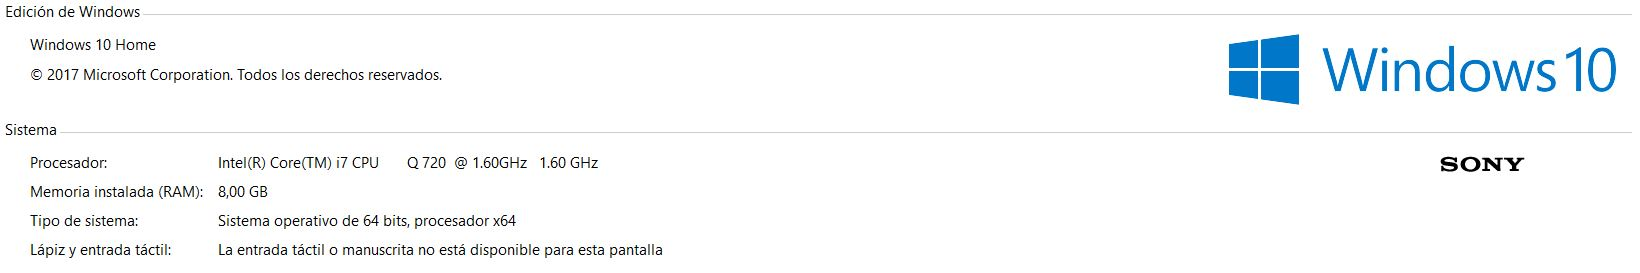
\includegraphics[width=1\textwidth]{/windows_ver}
		\caption{Información de Windows}
		\label{fig:winver}
	\end{center}
\end{figure}

\newpage

Del mismo modo, se ha usado un \textit{smartphone} para comprobar el correcto funcionamiento de la aplicación.

\begin{itemize}
	\item \textbf{Marca y modelo:} LG Optimus L5 II.
	\item \textbf{Procesador:} MediaTek MT6575 @ 1 \acs{GHz}.
	\item \textbf{RAM:} 1 \acs{GB}.
	\item \textbf{Memoria interna:} 4 \acs{GB}.
\end{itemize}

\subsection{Recursos Software}

\subsubsection*{Sistema Operativo}
Aunque, como se ha comentado anteriormente, se han usado diferentes ordenadores personales para desarrollar este trabajo, principalmente se ha usado Microsoft Windows 10 Home \cite{Microsoft}. En cuanto al \textit{smartphone}, se usará Android \cite{Andro}.

\subsubsection*{Lenguaje de Programación}
Puesto que la aplicación está destinada a \textit{smartphones} Android, el lenguaje de programación ha de ser Java. Java es un lenguaje de programación orientado a objetos usado para el desarrollo de aplicaciones cuyos propósitos son muy variados, puesto que también ofrece concurrencia \cite{Java}.

\subsubsection*{Android Studio}
Android Studio \cite{AndroidStudio} es el \acs{IDE} oficial para el desarrollo de aplicaciones en Android, proporcionando las herramientas necesarias para ello. Además, posee integración con \textit{Firebase}, lo que permite conectar las aplicaciones con este servicio para agregar \textit{Analytics}, \textit{Authentication} y \textit{Notifications}, entre otros servicios, que resultarán imprescindibles para el desarrollo de este trabajo.

\newpage

\subsubsection*{Firebase}
Firebase \cite{GooFirebase} es, principalmente, un \textit{backend} que facilita las tareas de programación en el lado del servidor, puesto que proporciona acceso fácil a los recursos que ofrece. No sólo ofrece soporte al desarrollo de aplicaciones en Android, sino que también está disponible para su integración en iOS y aplicaciones web. Algunas de sus funciones son:

\begin{itemize}
	\item \textbf{\textit{Cloud Firestore}}. Se trata de una base de datos en tiempo real, evolución de \textit{Realtime Database}. Ofrece una base de datos no relacional.
	\item \textbf{\textit{Authentication}}. Permite autenticar usuarios de forma simple en las aplicaciones de un proyecto. Además del usual método de entrada usando correo y contraseña, permite la autenticación mediante redes sociales y número de teléfono.
	\item \textbf{\textit{Remote Config}}. Permite modificar la aplicación de manera remota en todos los clientes in necesidad de implementar una nueva versión.
\end{itemize}

\subsubsection*{IBM Bluemix}
IBM Bluemix es una plataforma que permite el uso de utilidades \textit{cloud} de manera sencilla. Ofrece diversos servicios, entre los que se encuentra IBM Watson. Este servicio ofrece tecnologías cognitivas para crear aplicaciones inteligentes, aportando la posibilidad de analizar y comprender sentimientos o palabras claves a partir de un texto. Esto servirá de ayuda a la hora de interpretar si un mensaje es adecuado o no para su envío mediante \textit{Natural Languaje Understanding} \cite{IBM}.

\subsubsection*{LaTeX}
En cuanto a la documentación, se ha usado el lenguaje de generación de documentos \LaTeX{}, junto con la clase \esitfg{} proporcionada. \LaTeX{} es un sistema de preparación de documentos de alta calidad tipográfica usado principalmente en documentos técnicos o científicos y permite a los autores no preocuparse demasiado por la apariencia de estos documentos, permitiendo centrarse en el contenido \cite{TheLatexProject}.

% Local Variables:
%  coding: utf-8
%  mode: latex
%  mode: flyspell
%  ispell-local-dictionary: "castellano8"
% End: